\begin{abstract}
Can a recurrent difference between machine and human prose become a controllable model coordinate? We trace one corpus-conditioned realization signature through four linked tests: surface recurrence, cross-generator hidden readout, fixed-token causal transport, and free-generation realization. The signature is estimated from 500 matched English continuations under two elicitation interfaces and evaluated in Llama~3.1~8B and Qwen3~4B. Lexical and syntactic directions recur across generators and remain continuously readable when the evaluated generator is excluded from fitting. A source-consistent Jacobian pullback then gives lexical transport beyond every one of 100 complete fitted-pipeline nulls in both models (\(p=0.0099\)); syntax remains a readable comparison direction. Finally, a 20-prompt development set selects a single intervention magnitude before a held-out test on 166 untouched prompts and three paired decode seeds. In Llama, the lexical intervention produces a target projection of \(0.269\,[0.127,0.412]\) and component selectivity of \(0.287\,[0.117,0.459]\); all three seed means are positive, while syntactic and discourse off-target intervals cover zero. The result connects a distributed surface regularity to selective lexical control under a frozen, explicitly scoped intervention.
% 中文：机器文本与人类文本之间反复出现的差异，能否成为可控制的模型坐标？我们让一个依赖于语料的语言实现特征依次经过四项相连的检验：表面复现、跨生成器隐藏读出、固定 token 因果传输和自由生成实现。该特征由两种诱导接口下的 500 对匹配英文续写估计，并在 Llama 3.1 8B 与 Qwen3 4B 中评估。词汇和句法方向能够跨生成器复现；当被评估生成器完全不参与拟合时，两者仍可被连续读取。随后，来源一致的 Jacobian 回拉在两个模型中都产生了超过全部 100 个完整拟合流水线零假设的词汇传输（(p=0.0099)），而句法方向保留为可读取的比较方向。最后，我们先在 20 个开发提示上选择唯一的干预强度，再在 166 个未参与调参的提示和三个配对解码种子上进行持出检验。在 Llama 中，词汇干预得到 (0.269,[0.127,0.412]) 的目标投影与 (0.287,[0.117,0.459]) 的成分选择性；三个种子均值全部为正，而句法和篇章非目标区间覆盖零。该结果在一个冻结且明确限定范围的干预下，把分布式表面规律连接到了选择性词汇控制。
\end{abstract}

\begin{figure*}[t]
    \centering
    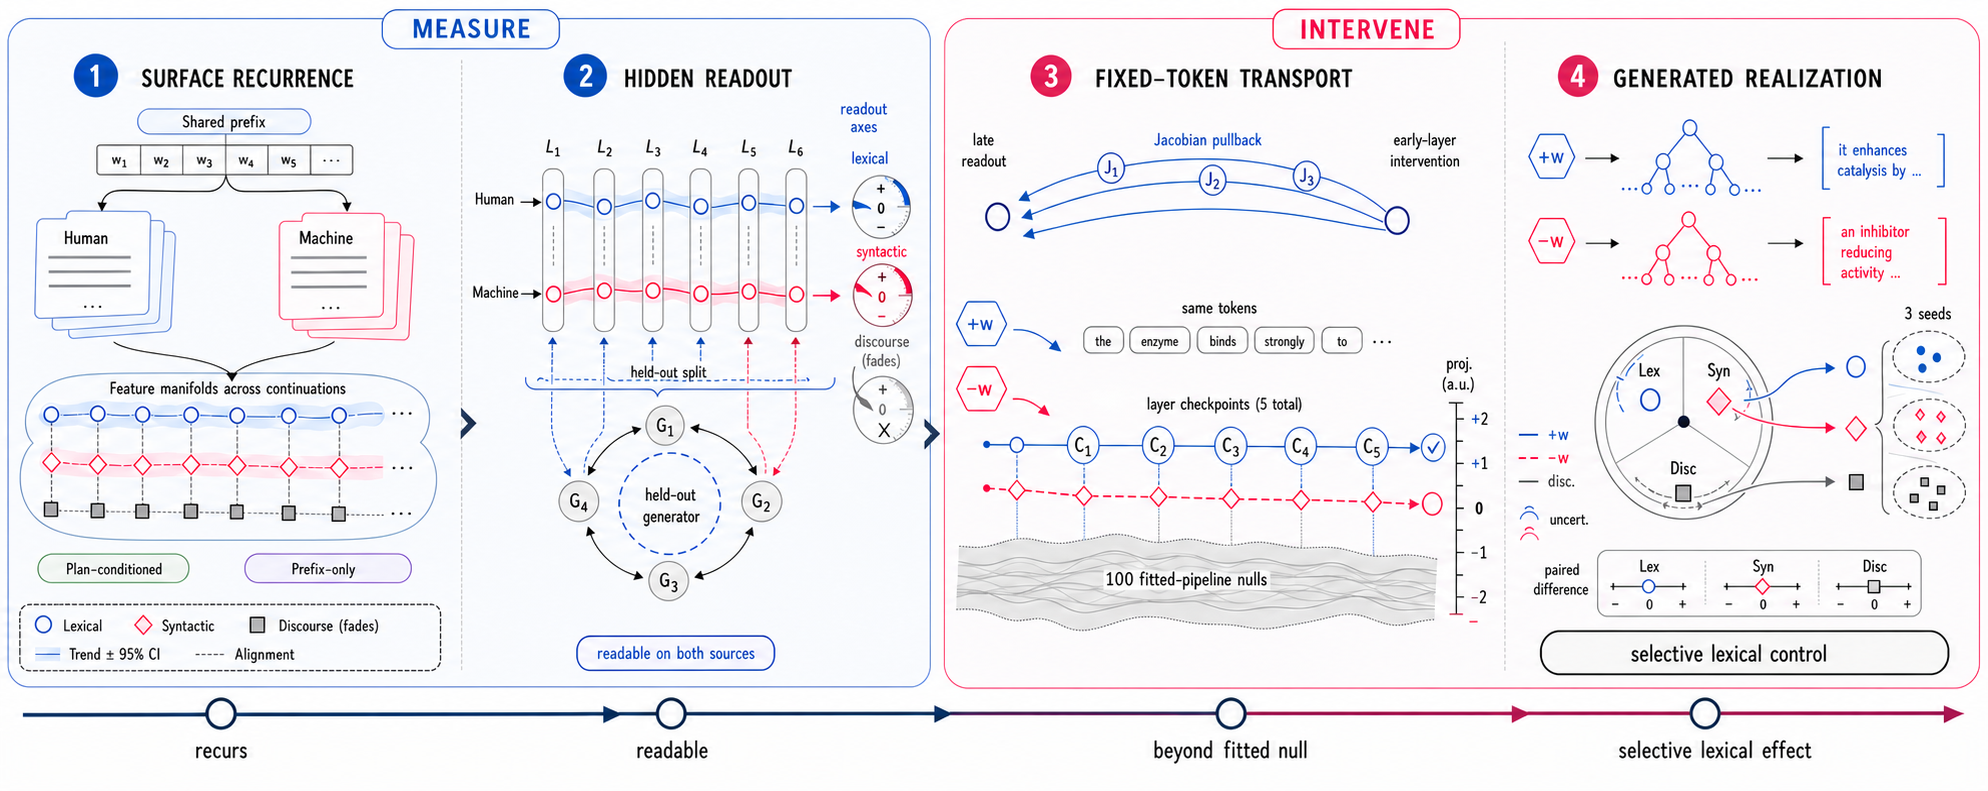
\includegraphics[width=\textwidth]{figures/main_overview.png}
    \caption{\textbf{From recurrence to selective realization.} Frozen surface axes are read across held-out generators, pulled back through model depth, tested against 100 refitted nulls, and evaluated in paired generation.}
    % 中文图注：从表面复现到选择性实现。冻结的表面轴先在留出生成器上读取，再沿模型深度回拉，与 100 个重拟合零假设比较，最终在配对生成中评估。
    \label{fig:main-overview}
\end{figure*}

\section{Introduction}
% 中文：引言

A human literary continuation asks, ``Why prematurely claim to have reached finality, when unexpected novelties may shatter any system before it is even completed?'' Its matched machine continuation states, ``Claiming finality is premature because unexpected novelties can shatter any system before completion.'' The proposition remains, but a rhetorical question becomes a declarative causal relation and the wording is regularized. We ask whether such recurring choices are merely visible at the surface or can be located and selectively moved inside a language model.
% 中文：一条人类文学续写问道：“既然意外的新事物可能在体系完成之前将其击碎，为什么要过早宣称体系已经终结？”匹配的机器续写则陈述：“宣称终结为时过早，因为意外的新事物可能在体系完成之前将其击碎。”命题保持不变，但反问被改写为陈述式因果关系，措辞也更加规则。我们要问的是，这类反复出现的选择是否只在表面可见，还是能够在语言模型内部被定位并选择性移动。

Prior work supplies the endpoints of this question but not the bridge between them. Linguistic analyses identify lexical, syntactic, and rhetorical contrasts in generated text \citep{zamaraeva2025comparing,zanotto2025profiling,reinhart2025variation}; representation methods recover linguistic information from model states \citep{hewitt2019probe}; and activation interventions alter model behavior \citep{rimsky2024caa}. A surface regularity, an accessible hidden coordinate, and a realized output effect are nevertheless different objects. Connecting them requires keeping the linguistic construct fixed while the evidence changes from observation to intervention.
% 中文：既有工作提供了这一问题的两个端点，却没有建立二者之间的桥梁。语言学分析识别生成文本中的词汇、句法和修辞差异；表征方法从模型状态中恢复语言信息；激活干预则改变模型行为。然而，表面规律、可访问的隐藏坐标和最终输出效应仍是不同对象。要把它们连接起来，就必须在证据从观察转向干预时始终固定同一个语言构念。

We define a \emph{machine--human realization signature}: a corpus-conditioned direction over recurrent wording and clause-structure choices in continuations of the same natural context. The signature is estimated from 500 matched pairs under a proposition-conditioned interface, then challenged on a prefix-only interface that removes the human-derived plan. This design asks whether a distributed realization pattern survives both generator variation and a change in elicitation, rather than turning familiar words into an authorship detector.
% 中文：我们定义“机器—人类语言实现特征”：在延续同一自然语境时，由反复出现的措辞与从句结构选择构成、依赖于语料的方向。该特征先由命题条件接口下的 500 对匹配文本估计，再转移到移除人类命题计划的纯前缀接口上检验。该设计关注分布式语言实现模式能否经受生成器变化与诱导方式变化，而不是把熟悉的词汇变成作者身份检测器。

Figure~\ref{fig:main-overview} turns this question into a four-stage evidence chain. We first establish recurrence of frozen lexical and syntactic axes across generators, domains, and interfaces. We then train continuous readouts while withholding an entire generator and require prediction on both human and machine continuations. Next, a source-consistent Jacobian pullback maps the late lexical readout to an early intervention and compares its five-checkpoint transport curve with 100 null pipelines that repeat every fitting step after permuting only the linguistic correspondence. Finally, we freeze the lexical pole and intervention site, select one magnitude on 20 development prompts, and test target-aligned, component-selective realization on 166 untouched prompts with three paired seeds.
% 中文：图~\ref{fig:main-overview} 把这一问题组织成四阶段证据链。首先，我们检验冻结的词汇与句法轴能否跨生成器、领域和接口复现。随后，在完整留出一个生成器的情况下训练连续读出器，并要求其在人类续写和机器续写两侧都能预测得分。接着，来源一致的 Jacobian 回拉把后期词汇读出映射为早期干预，并将五检查点传输曲线与 100 条完整零流水线比较；这些零流水线重复全部拟合步骤，只打乱语言得分与样本的对应关系。最后，我们冻结词汇极性和干预位置，只在 20 个开发提示上选择一次强度，再使用 166 个未参与调参的提示和三个配对随机种子检验目标一致且具有成分选择性的语言实现。

The lexical direction passes all four stages. It recurs under both interfaces, remains readable for every held-out generator, and exceeds all refitted transport nulls in both Llama and Qwen. In the final Llama test, the \(+10\%/-10\%\) intervention shifts the lexical score by \(0.269\,[0.127,0.412]\) and exceeds the mean off-target response by \(0.287\,[0.117,0.459]\). The effect is positive in every seed; its target-minus-syntax and target-minus-discourse contrasts are also positive. Thus the same lexical construct is observable at the surface, readable in hidden states, causally transportable on fixed sequences, and selectively realizable in sampled text.
% 中文：词汇方向通过了全部四个阶段。它在两种接口下都能复现，对每个留出生成器都保持可读取，并且在 Llama 与 Qwen 中都超过全部重拟合传输零假设。在最终的 Llama 检验中，(+10\%/-10\%\) 干预使词汇得分移动 (0.269,[0.127,0.412])，并以 (0.287,[0.117,0.459]) 超过非目标响应均值。三个种子中的效应全部为正，目标减句法和目标减篇章的对比也都为正。因此，同一个词汇构念能够在表面被观察、在隐藏状态中被读取、在固定序列上被因果传输，并在采样文本中被选择性实现。

The contribution is deliberately specific. The final selective-generation result concerns the lexical axis in Llama at a development-selected single-layer strength; syntax remains a comparison axis and the earlier 5\% multi-condition audit is reported as sensitivity evidence. Within that scope, the result provides an end-to-end account of how a distributed linguistic signature can become a controllable coordinate rather than stopping at detection or probing.
% 中文：本文的贡献具有明确范围。最终的选择性生成结果只针对 Llama 中的词汇轴，并使用开发集选择的单层干预强度；句法轴保留为比较方向，较早的 5% 多条件审计则作为敏感性证据报告。在这一范围内，本文给出了一个端到端解释：分布式语言特征如何成为可控制坐标，而不是停留在检测或探针层面。

Table~\ref{tab:estimands-at-glance} summarizes the changing evaluation unit from held-out generators to fixed sequences, refitted pipelines, and held-out prompt-level effects.
% 中文：表~\ref{tab:estimands-at-glance} 汇总了评估单位如何从留出生成器依次转向固定序列、重拟合流水线和持出提示级效应。

\begin{table*}[!tbp]
\centering
\maintablefont
\setlength{\tabcolsep}{5pt}
\renewcommand{\arraystretch}{1.10}
\begin{tabular}{@{}
  >{\raggedright\arraybackslash}p{0.12\textwidth}
  >{\raggedright\arraybackslash}p{0.16\textwidth}
  >{\raggedright\arraybackslash}p{0.64\textwidth}@{}}
\toprule
\textbf{Stage} & \textbf{Estimand} & \textbf{Construction and evaluation}\\
\midrule
Surface & Axis \(u_g\) &
500 paired feature differences; \(\Delta\), paired \(d\), and FDR \(q\).\\
Readout & Cross-generator \(D\) &
Three-generator train, one-generator test; Pearson \(r\) on both sources.\\
Pullback & Canonical \(w\) &
32 balanced Jacobian pairs; source-side agreement and frozen-anchor response.\\
Trace & Capacity \(C\) &
Five intermediate checkpoints on 100 identical fixed sequences.\\
Null test & Curve \(p_{\mathrm{null}}\) &
100 complete pipeline refits and an add-one curve-statistic rank.\\
\multirow[c]{2}{*}[-0.55ex]{Generation} & Target \(p_g\) &
Paired \(+\alpha/-\alpha\) generations; strength selected on 20 development prompts and tested on 166 untouched prompts.\\
\graycmidrule{2-3}
& Selectivity \(b_g\) &
Target response minus the mean of two off-target responses.\\
\bottomrule
\end{tabular}
\caption{\textbf{Evidence-chain estimands.} Units progress from held-out generators to fixed sequences, refitted pipelines, and held-out prompt effects.}
% 中文表注：证据链估计量。评估单位从留出生成器推进到固定序列、重拟合流水线与持出提示效应。
\label{tab:estimands-at-glance}
\end{table*}

\section{Related Work}
% 中文：相关工作

\subsection{Surface Signals}
% 中文：表面信号

Machine and human text differ in vocabulary, dependency structure, and discourse organization, although the reported cues vary across models and domains \citep{munozortiz2024contrasting,elattar2026systematic,ahmad2026human}. Detector failures under distribution shift show why these cues should not be treated as universal authorship rules \citep{sadasivan2024detection,li-etal-2024-mage,shamardina2025coat}. We instead define a corpus-conditioned multivariate direction and ask whether it recurs across named generators, domains, and elicitation interfaces.
% 中文：机器文本与人类文本在词汇、依存结构和篇章组织上存在差异，但不同模型与领域报告的线索并不一致。检测器在分布变化下的失败说明，这些线索不应被当作普适的作者身份规则。本文改为定义一个依赖于语料的多变量方向，并检验它能否在具名生成器、领域和诱导接口之间复现。

\subsection{Representation Readout}
% 中文：表征读出

Representation-based detectors can separate human and generated text from observer-model states \citep{chen-etal-2025-repreguard,vishnyakov2026svdetect}. Our readout carries a different burden: it predicts an independently measured continuous linguistic score on both sides of the source contrast, with the evaluated generator excluded from every fit. Positive human/machine agreement is required before the two source-side patterns form a consensus direction, so a source-only boundary cannot by itself satisfy the test.
% 中文：基于表征的检测器可以利用观察模型的状态区分人类文本和生成文本。本文的读出器承担不同的任务：它需要预测来源对比两侧独立测量的连续语言得分，并且被评估的生成器必须从所有拟合步骤中排除。只有在人类侧与机器侧的模式呈正向一致时，二者才能组成共识方向，因此仅仅存在来源分类边界并不足以通过检验。

\subsection{Causal Intervention}
% 中文：因果干预

Probes test whether information is accessible, whereas causal use requires intervention evidence \citep{hewitt2019probe}. Activation addition controls varied behaviors \citep{turner2023activation,rimsky2024caa,li2023iti}, but reliability depends on readout--behavior alignment, specificity, and direction identifiability \citep{canby2025reliable,waldis2026aligned,goyal2026specificity,venkatesh2026nonidentifiability}. Nullspace and amnesic methods further show that an intervention's meaning depends on the variation it removes \citep{ravfogel2020inlp,elazar2021amnesic}. Together, these literatures motivate separate tests of surface recurrence, hidden readability, fixed-token transport, and generated-language realization. We apply those tests in sequence to one fixed linguistic construct.
% 中文：探针检验信息是否可访问，而因果使用还需要干预证据。激活加法可以控制多种行为，但其可靠性取决于读出器与行为的对齐、特异性以及方向的可识别性。零空间与遗忘式方法也表明，干预的含义取决于它移除了哪类变异。综合来看，这些研究促使我们分别检验表面复现、隐藏可读性、固定 token 传输和生成语言实现；本文把这些检验依次应用于同一个固定的语言构念。

Our setting therefore sits between computational stylistics and mechanistic intervention. Surface studies supply a measurable linguistic construct, but distribution-shift failures caution against turning it into a detector; representation methods supply candidate coordinates, but accessibility alone does not establish functional use; steering methods supply an intervention, but output change must be aligned with the construct that motivated it. Keeping the same score fixed across these interfaces lets each literature contribute a distinct evidential link instead of allowing success at one link to rename the claim at the next.
% 中文：因此，本文位于计算文体学与机制干预之间。表面研究提供可测量的语言构念，但分布变化下的失败提醒我们不能把它直接变成检测器；表征方法提供候选坐标，但可访问性本身不能建立功能使用；激活引导方法提供干预，但输出变化必须与最初定义该方向的构念对齐。在这些接口之间固定同一个得分，使每类研究分别贡献一个证据环节，而不会让某一环节的成功自动改写下一环节的主张。

\section{Method}
\label{sec:method}
% 中文：方法

\subsection{Surface Signature}
\label{sec:construct}
% 中文：表面语言特征

\paragraph{Two interfaces.} The proposition-conditioned corpus contains 500 English continuation pairs balanced across PG-19, WikiLingua, Wikipedia, and XL-Sum \citep{rae2020compressive,ladhak2020wikilingua,wikimedia2023wikipedia,hasan2021xlsum}. A planner extracts a proposition plan from each human continuation, a distinct generator continues the natural prefix from that plan, and a third model checks coverage and contradiction. The prefix-only corpus regenerates the same 500 samples from the prefix and target length alone. Mean semantic cosine is 0.925 under proposition conditioning and 0.727 under prefix-only generation, compared with 0.469 after within-source derangement. The proposition-conditioned interface provides stronger content control, whereas the prefix-only interface removes the asymmetric plan-to-text channel. Section~\ref{app:corpus-detail} records construction, rejection, and leakage audits.
% 中文：两种互补接口。命题条件语料包含 500 对英文续写，并在 PG-19、WikiLingua、Wikipedia 与 XL-Sum 之间保持平衡。规划模型从每条人类续写中提取命题计划，独立的生成器依据该计划延续自然前缀，第三个模型检查内容覆盖与矛盾。纯前缀语料则只根据前缀和目标长度重新生成同一组 500 个样本。命题条件接口的平均语义余弦为 0.925，纯前缀接口为 0.727，而来源内部错配后的基线为 0.469。命题条件接口提供更强的内容控制，而纯前缀接口移除了不对称的计划到文本通道。第~\ref{app:corpus-detail} 节记录了构建、拒绝和泄漏审计。

The two arms are not interchangeable replications; they expose opposite sources of uncertainty. Proposition conditioning makes content mismatch a less plausible explanation, but the machine alone receives the explicit plan and may lexicalize its structure. Prefix-only generation removes that route, but allows larger semantic divergence. We therefore fit every axis and readout only on the proposition-conditioned arm and treat prefix-only text as an untouched transfer environment. Recurrence across the two arms cannot establish content-invariant authorship, but it is harder to attribute solely to either plan verbalization or unconstrained topic drift.
% 中文：两个分支并不是可以互换的重复实验，而是暴露了相反的不确定性来源。命题条件使内容不匹配成为较不可信的解释，但只有机器文本接收显式计划，因此可能把计划结构词汇化。纯前缀生成移除了这一路径，却允许更大的语义偏离。因此，所有轴与读出器都只在命题条件分支上拟合，纯前缀文本则作为完全未参与拟合的迁移环境。两个分支之间的复现不能建立与内容无关的作者身份，但更难仅仅归因于计划表述或无约束的主题漂移。

Sample selection is frozen before linguistic measurement. All 500 accepted proposition-conditioned pairs pass an independent automatic judge, use distinct planner, generator, and judge models, and receive no post-generation repair. Their machine--human length ratio has mean 0.935 and median 0.925, with range 0.603--1.405; length and six further nuisance statistics are nevertheless removed inside every training fold. These controls do not certify rhetorical equivalence, but they prevent the surface construct from being defined by obvious selection, repair, or length asymmetries.
% 中文：样本选择在语言测量之前冻结。全部 500 对已接受的命题条件样本都通过独立自动评审，每对都使用彼此不同的规划器、生成器与评审器，并且不进行生成后修补。机器—人类长度比的均值为 0.935，中位数为 0.925，范围为 0.603--1.405；尽管如此，长度以及另外六个干扰统计量仍在每个训练折内部被移除。这些控制不能证明修辞等价，却能避免表面构念由明显的选择、修补或长度不对称所定义。

\paragraph{Frozen directions.} We predefine 35 measurements: 10 lexical, 12 syntactic, and 13 discourse features. Seven length, entity, and number statistics are nuisance variables rather than target features. Each training fold residualizes the linguistic measurements against those nuisances, standardizes them, and projects them onto the paired machine-minus-human direction. Lexical and syntactic axes are confirmatory targets; discourse remains an off-target audit because it fails the same stability gate. The full dictionary, fold construction, PCA sensitivity, and same-token vocabulary analysis are reported in Sections~\ref{app:features} and~\ref{app:concordance}.
% 中文：冻结的语言方向。我们预先定义 35 个测量，其中包括 10 个词汇特征、12 个句法特征和 13 个篇章特征。另有 7 个长度、实体和数字统计量作为干扰变量，而不是目标特征。每个训练折先用这些干扰变量对语言测量进行残差化和标准化，再把它们投影到配对的机器减人类方向上。词汇轴和句法轴是验证性目标；篇章轴未通过相同的稳定性门槛，因此仅作为非目标审计。完整特征字典、折内构造、PCA 敏感性和同 token 词汇分析见第~\ref{app:features} 节和第~\ref{app:concordance} 节。

The construction treats the signature as a distributed relation rather than a list of diagnostic words. Grouping measurements before analysis prevents a conspicuous cue from defining the target after outcomes are known, while fold-local nuisance removal prevents length, entity density, or number density from becoming shortcuts. The paired direction then asks which combination of residualized choices changes consistently between continuations of the same context. This design makes lexical and syntactic scores interpretable as degrees of realization within the observed corpus; it does not convert any individual feature into an authorship rule.
% 中文：这一构造把该特征视为一种分布式关系，而不是诊断词汇清单。事先划分测量组，可以避免在观察结果后由某个显眼线索反过来定义目标；折内移除干扰变量，则防止长度、实体密度或数字密度成为捷径。随后，配对方向检验的是：在延续同一语境时，哪些经过残差化的语言选择组合会在人类文本与机器文本之间持续变化。因此，词汇和句法得分可以解释为观测语料内部语言实现程度的差异，但任何单个特征都不会因此成为作者身份规则。

\begin{figure*}[t]
    \centering
    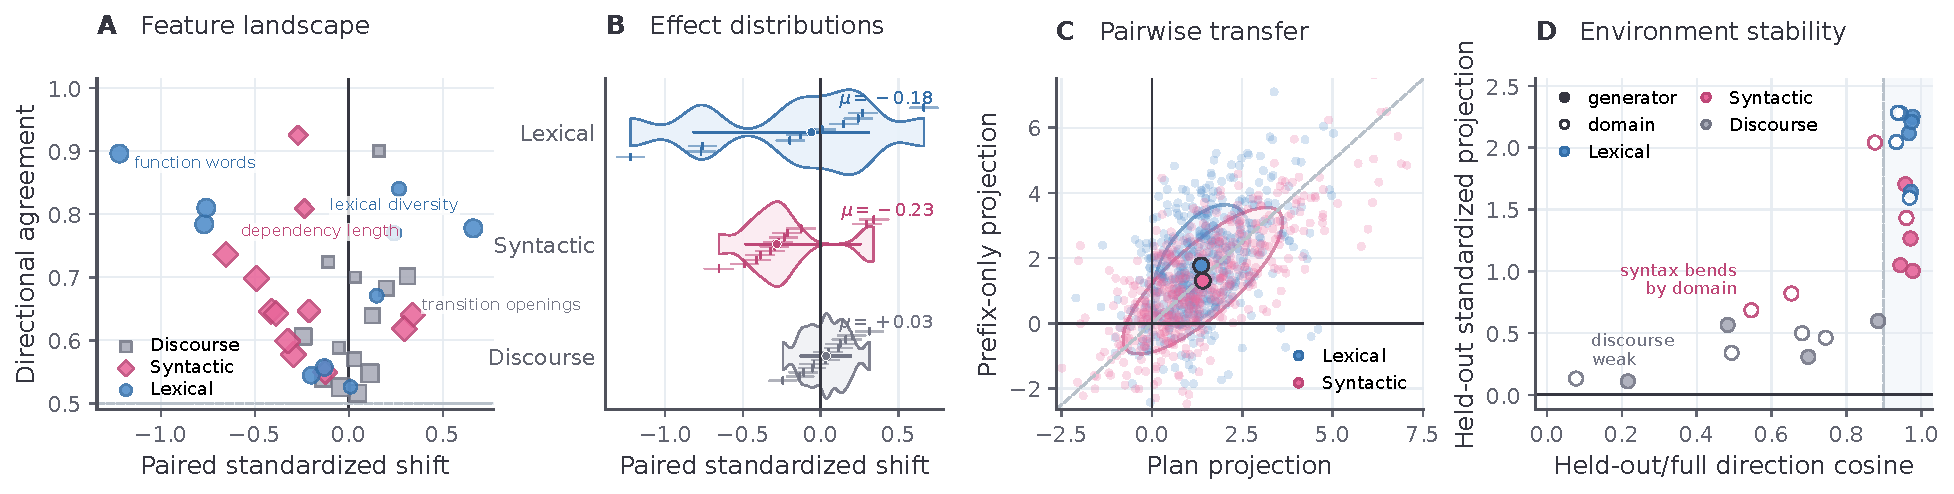
\includegraphics[width=\textwidth]{figures/machine_signature_atlas.pdf}
    \caption{\textbf{Lexical and syntactic directions recur across environments.} (A) Feature shifts. (B) Group effects. (C) Interface transfer. (D) Generator and domain holdouts.}
    % 中文图注：词汇与句法方向能够跨环境复现。(A) 特征位移；(B) 组级效应；(C) 接口迁移；(D) 生成器和领域留出。
    \label{fig:signature}
\end{figure*}

\subsection{Hidden Readout}
% 中文：隐藏读出

Let \(h_i^k\) be the mean continuation state after block \(k\), projected away from the leading ten pooled within-class nuisance directions. For each held-out generator and source side, we fit a forward covariance pattern between these states and the frozen surface score. Human and machine patterns must have positive cosine before their normalized sum defines the cross-generator readout \(v_g^k\). Every nuisance fit, surface direction, and hidden pattern excludes the evaluated generator. The readout is successful only if it predicts the continuous score on both human and machine continuations, rather than merely separating their sources.
% 中文：令 \(h_i^k\) 表示第 \(k\) 个模块之后的续写平均状态，并移除合并的类内干扰方向中排名最前的十个方向。针对每个留出生成器和来源侧，我们拟合隐藏状态与冻结表面得分之间的前向协方差模式。只有当人类侧和机器侧模式的余弦为正时，它们的归一化和才定义跨生成器读出方向 \(v_g^k\)。所有干扰拟合、表面方向和隐藏模式都排除被评估的生成器。读出器必须在人类续写和机器续写上都能预测连续得分，而不能只区分来源。
\begin{equation}
\begin{aligned}
\widetilde v_{ga}^k&=H_a^\top z_{ga}/(z_{ga}^\top z_{ga}), &
v_{ga}^k&=\operatorname{unit}(\widetilde v_{ga}^k),\\
v_g^k&=\operatorname{unit}(v_{g,h}^k+v_{g,m}^k), && a\in\{h,m\}.
\end{aligned}
\label{eq:covariance-readout}
\end{equation}

The readout stage tests generalization of the declared linguistic variable, not merely separability of human and machine sources. A source classifier could exploit a generator-specific artifact while remaining unrelated to the frozen realization score. Continuous prediction within both source sides instead asks whether the same hidden direction orders human and machine continuations by independently measured realization, and excluding the evaluated generator asks whether that relation survives a new generator environment. Positive held-out correlations therefore establish accessibility of the declared surface variable under generator transfer; they do not yet show that an early intervention transports it through the model.
% 中文：读出阶段检验的是已声明语言变量的泛化，而不只是人类文本与机器文本是否可分。来源分类器可能利用生成器特有的人为线索，却与冻结的语言实现得分无关。要求在人类侧和机器侧分别预测连续得分，是在检验同一个隐藏方向能否按照独立测量的语言实现程度排列两侧续写；排除被评估生成器，则检验这种关系能否迁移到新的生成器环境。因此，正的留出相关只能证明该表面变量在跨生成器条件下可访问，还不能证明早期干预会把它传过模型。

The opening literary pair interprets the surface construct, while the held-out continuous test establishes its hidden-state generalization. This division of labor is important: examples reveal what movement along the direction looks like, and generator-level holdout verifies that the readout orders many unseen human and machine continuations by the same independently measured score.
% 中文：开篇的文学样本对负责解释表面构念，而留出连续检验负责建立其隐藏状态泛化。二者分工明确：例子展示沿该方向移动在语言上是什么样子，生成器级留出则验证读出器能否按照同一个独立测量得分，对大量未见的人类与机器续写进行排序。

\subsection{Fixed-Token Transport}
% 中文：固定 token 传输

Earlier residual streams use different coordinates from the late readout. For source side \(a\), we translate the readout backward through the layer-to-layer Jacobian and combine the independently estimated human and machine pullbacks only after projecting through the frozen nuisance-nullspace projector \(P_m\):
% 中文：较早层的残差流与后期读出器使用不同坐标。对于来源侧 \(a\)，我们通过层间 Jacobian 将读出方向向前层回拉，并在经过冻结的干扰零空间投影器 \(P_m\) 后，才组合独立估计的人类侧和机器侧回拉方向：
\begin{equation}
\begin{aligned}
a_{ig}^{a}&=(J_i^{\ell\rightarrow k})^\top v_g^k,\\
\hat a^a&=\operatorname{unit}(P_m\bar a^a),\\
w_{mg}&=\operatorname{unit}(\hat a^\human+\hat a^\machine).
\end{aligned}
\label{eq:pullback-main}
\end{equation}

Applying the late readout vector directly at an early layer would assume that residual coordinates retain the same meaning across depth. The Jacobian transpose instead maps sensitivity of the declared late readout into the early residual space, so each fitted sequence contributes a local first-order pullback rather than an untransformed activation direction. Human and machine pullbacks are estimated separately, projected through the same frozen nuisance nullspace, and combined without outcome-dependent sign correction. This construction yields a preoriented early direction for the fixed-token test, but it does not optimize the surface form of sampled continuations.
% 中文：如果把后期读出向量直接施加到早期层，就等于假设残差坐标在网络深度之间保持相同含义。Jacobian 转置则把已声明后期读出器的敏感度映射回早期残差空间，使每条拟合序列贡献一个局部一阶回拉方向，而不是直接复用未经转换的激活方向。人类侧与机器侧回拉分别估计，经过同一个冻结干扰零空间投影，并且不会根据生成结果事后翻转符号。这个构造为固定 token 检验提供了预先定向的早期方向，但它并没有优化采样续写的表面形式。

The source-side signs are retained, so \(+w\) is oriented by the machineward readout before any generation outcome is observed. On an unchanged token sequence, symmetric \(+w/-w\) intervention measures the signed response of the late readout; its absolute value is the transport capacity. The confirmatory statistic is the depth-normalized area over five intermediate checkpoints, excluding the injection layer and fitted readout anchor because both are construction-internal.
% 中文：来源侧的符号保持不变，因此在观察任何生成结果之前，\(+w\) 的极性已经由机器方向的读出器确定。在不变的 token 序列上，对称的 \(+w/-w\) 干预测量后期读出器的有符号响应，其绝对值定义传输容量。验证性统计量是五个中间检查点上的深度归一化面积；注入层和拟合读出锚点都属于构造内部位置，因此被排除。
\begin{equation}
\begin{aligned}
\tau_{img}(w)&=\frac{(h_i^k(+\alpha w)-h_i^k(-\alpha w))^\top v_g^k}{2\alpha\lVert w\rVert_2},\\
\widehat C_{mgj}&=\frac{1}{n}\sum_i\lvert\tau_i(w_{mg},v_g^j)\rvert,\\
\widehat C^0_{mgj}&=\frac{1}{R}\sum_r\left[\frac{1}{n}\sum_i\lvert\tau_i(w_{mgr},v_{gr}^j)\rvert\right].
\end{aligned}
\label{eq:transport-response}
\end{equation}

The comparison is a complete fitted-pipeline null, not a random input direction. Each of \(R=100\) replicates permutes surface scores within corpus--generator strata, refits every layerwise readout, reconstructs the source-consistent pullback, and intervenes on the same 100 hashed sequences. The add-one rank \(p=(1+\#\{T_r^0\geq T\})/(R+1)\) asks whether the learned depth profile is unusual when every fitting advantage is retained but the linguistic correspondence is broken. Section~\ref{app:direction-detail} gives the complete estimands, layer conventions, trajectory checks, and sensitivity settings.
% 中文：比较对象是完整拟合流水线零假设，而不是随机输入方向。\(R=100\) 个重复中的每一个都会在语料—生成器分层内打乱表面得分，重新拟合每一层读出器，重建来源一致的回拉方向，并在相同的 100 条哈希序列上进行干预。加一排序 \(p=(1+\#\{T_r^0\geq T\})/(R+1)\) 检验：当所有拟合优势都被保留、只有语言对应关系被破坏时，学习到的深度轨迹是否仍然异常。第~\ref{app:direction-detail} 节给出完整估计量、层编号、轨迹检查与敏感性设置。

\subsection{Generated-Language Realization}
% 中文：生成语言实现

Fixed-token transport measures a late readout along an unchanged trajectory; free generation asks whether that coordinate survives autoregressive feedback. We separate strength selection from evaluation. A disjoint 20-prompt development set (indices 0--19) compares candidate magnitudes while keeping the lexical pole, L7 intervention site, token budget, and decoding rule fixed. The selected endpoint, \(\alpha=2\), equals 10\% of the mean hidden-state norm. We then freeze the complete protocol and evaluate prompts 34--199: 166 untouched prompts under three paired decode seeds. For measurement group \(g\), target projection \(p_{ig}\) and component selectivity \(b_{ig}\) are
% 中文：固定 token 传输沿不变轨迹测量后期读出，而自由生成检验该坐标能否经受自回归反馈。我们将强度选择与最终评估分开。在互不重叠的 20 个开发提示（索引 0--19）上比较候选强度，同时固定词汇极性、L7 干预位置、token 预算与解码规则。选中的端点为 \(\alpha=2\)，相当于平均隐藏状态范数的 10\%。随后冻结完整协议，并在索引 34--199 上进行评估：166 个未参与调参的提示，配合三个配对解码种子。对测量组 \(g\)，目标投影 \(p_{ig}\) 与成分选择性 \(b_{ig}\) 定义如下：
\begin{equation}
\begin{aligned}
p_{ig}(w)&=s_g(Y_i^{+w})-s_g(Y_i^{-w}),\\
b_{ig}(w)&=p_{ig}(w)-\frac{1}{2}\sum_{c\neq g}p_{ic}(w).
\end{aligned}
\label{eq:selectivity}
\end{equation}
The formal test uses 128 new tokens, temperature 0.7, top-\(p=0.95\), and base seed 8236. For each prompt, we compute the paired \(+\alpha/-\alpha\) difference in each seed, average the three differences within prompt, and bootstrap the 166 prompt means. The earlier 5\% one-seed matrix and multi-condition replication are retained in Section~\ref{app:seed-detail} as low-dose sensitivity evidence rather than used to estimate the formal effect.
% 中文：正式检验使用 128 个新 token、温度 0.7、top-\(p=0.95\) 和基础随机种子 8236。对每个提示，我们先计算每个种子下配对的 \(+\alpha/-\alpha\) 差值，再在提示内部平均三个差值，并对 166 个提示均值进行 bootstrap。较早的 5\% 单种子矩阵与多条件复现实验保留在第~\ref{app:seed-detail} 节中，作为低剂量敏感性证据，而不用于估计正式效应。

Target projection asks whether the output moves along the declared lexical axis; component selectivity asks whether that movement exceeds the mean syntactic and discourse response. We additionally test lexical-minus-syntactic and lexical-minus-discourse contrasts separately and report seed means alongside prompt-clustered intervals. This hierarchy makes selective realization a joint claim: the target effect, aggregate selectivity, and both pairwise contrasts must point in the declared direction.
% 中文：目标投影检验输出是否沿已声明的词汇轴移动；成分选择性检验这一移动是否超过句法与篇章响应的均值。我们还分别检验词汇减句法和词汇减篇章对比，并在按提示聚类的区间之外报告各随机种子均值。由此，选择性实现成为一个联合主张：目标效应、总体选择性与两个成对对比都必须指向预先声明的方向。

\section{Experiments}
\label{sec:experiments}
% 中文：实验设置

\paragraph{Models and splits.} We evaluate hidden readout and intervention in \llamamodel{} and \qwenmodel{}. Surface axes and readouts are fitted only on the proposition-conditioned corpus. Generator transfer follows a four-fold leave-one-generator-out design, while the prefix-only corpus remains untouched until transfer evaluation.
% 中文：模型与数据划分。我们在 \llamamodel{} 和 \qwenmodel{} 中评估隐藏读出与干预。表面方向和读出器只在命题条件语料上拟合。生成器迁移采用四折留一生成器设计，纯前缀语料则在迁移评估前始终不参与拟合。

\paragraph{Evaluation protocol.} Readout is evaluated separately on held-out human and machine continuations. Fixed-token transport uses 100 identical sequences, five intermediate checkpoints, and 100 complete fitted-pipeline null refits. Generated-language realization selects the lexical strength on 20 development prompts, then uses 166 disjoint test prompts with paired \(\pm2w\) outputs, three decode seeds, and prompt-clustered bootstrap intervals. Table~\ref{tab:estimands-at-glance} summarizes the estimands; Sections~\ref{app:direction-detail} and~\ref{app:seed-detail} give the frozen settings.
% 中文：评估协议。读出器分别在人类与机器的留出续写上评估。固定 token 传输使用 100 条完全相同的序列、五个中间检查点和 100 次完整拟合流水线零假设重拟合。生成语言实现先在 20 个开发提示上选择词汇干预强度，再使用 166 个互不重叠的测试提示生成配对的 \(\pm2w\) 输出，配合三个解码种子与按提示聚类的 bootstrap 区间。表~\ref{tab:estimands-at-glance} 汇总估计量；第~\ref{app:direction-detail} 节和第~\ref{app:seed-detail} 节给出冻结设置。

\section{Results}
\label{sec:results}
% 中文：结果

\begin{figure}[!t]
    \centering
    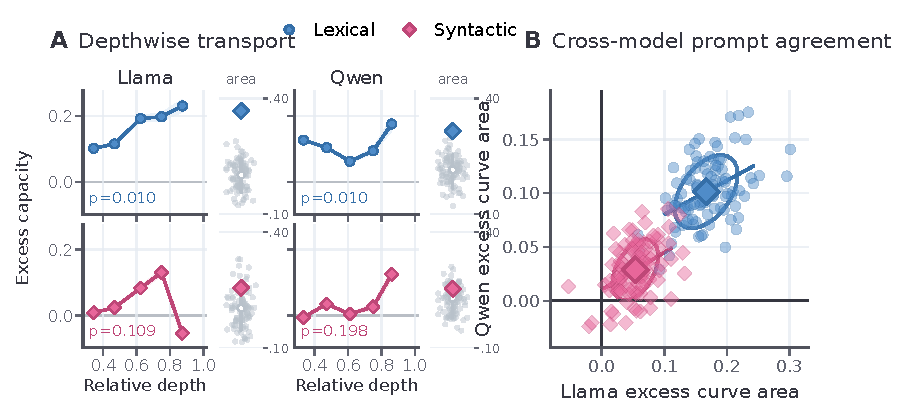
\includegraphics[width=\columnwidth]{figures/hidden_causal_trace.pdf}
    \caption{\textbf{Lexical transport exceeds the fitted-pipeline null in both models.} (A) Five-checkpoint excess capacity. (B) Prompt-level excess area.}
    % 中文图注：词汇传输在两个模型中均超过拟合流水线零假设。(A) 五检查点超额容量；(B) 提示级超额面积。
    \label{fig:hidden-trace}
\end{figure}

\paragraph{Surface recurrence.} Figure~\ref{fig:surface-summary} separates feature magnitude from cross-environment stability. The six largest paired effects span both confirmatory groups; lexical and syntactic directions remain aligned under every generator holdout and on the untouched prefix-only corpus. All three group-level sign-flip tests yield \(p=0.0002\); prefix-only transfer is confirmatory for the lexical and syntactic axes. Syntax bends more under domain holdout, while discourse is unstable and remains off-target. Figure~\ref{fig:realization-examples} grounds the directions in paired excerpts, and Figure~\ref{fig:app-surface-transfer} reports the plan-removal transfer.
% 中文：图~\ref{fig:surface-summary} 将特征效应大小与跨环境稳定性分开呈现。最大的六个配对效应跨越两个验证性特征组；词汇和句法方向在每个生成器留出条件以及未参与拟合的纯前缀语料上都保持同向。三个组级符号翻转检验均得到 \(p=0.0002\)；纯前缀迁移只对词汇轴与句法轴进行验证性检验。句法方向在领域留出下弯曲得更多，而篇章方向不稳定，因此仍作为非目标测量。图~\ref{fig:realization-examples} 用配对摘录解释这些方向，图~\ref{fig:app-surface-transfer} 报告移除计划后的迁移。

\begin{figure}[tbp]
\centering
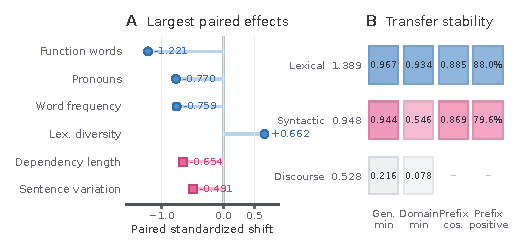
\includegraphics[width=\columnwidth]{figures/surface_result_summary.pdf}
\caption{\textbf{Surface recurrence is distributed and environment-tested.} (A) Six largest paired shifts. (B) Group shift, worst generator/domain agreement, and prefix-only transfer. Circles are lexical and squares syntactic.}
% 中文图注：表面复现具有分布式结构，并经过跨环境检验。(A) 最大的六个配对位移；(B) 组级位移、最弱生成器与领域一致性以及纯前缀迁移。圆点表示词汇特征，方块表示句法特征。
\label{fig:surface-summary}
\end{figure}

The abstract direction has visible linguistic content without reducing to a shibboleth. Across the matched corpus, \emph{however} occurs in 83 machine continuations and 34 human continuations, and \emph{despite} in 36 and 7. The evaluative forms \emph{crucial} and \emph{significant} each occur in 22 machine documents but 3 human documents; \emph{stated that} and \emph{noted that} occur in 16 and 13 machine documents and no matched human document. These counts help interpret the multivariate projection, but the direction is defined by the frozen distributed inventory rather than any one expression.
% 中文：这一抽象方向具有可见的语言内容，却不能被简化为某个刻板词汇。在匹配语料中，\emph{however} 分别出现在 83 条机器续写和 34 条人类续写中，\emph{despite} 分别为 36 与 7 条。评价性形式 \emph{crucial} 和 \emph{significant} 都出现在 22 篇机器文本中，却仅出现在 3 篇人类文本中；\emph{stated that} 与 \emph{noted that} 分别出现在 16 和 13 篇机器文本中，而未出现在任何匹配人类文本中。这些计数有助于解释多变量投影，但该方向由冻结的分布式指标库定义，而不是由任何单一表达定义。

The two transfer tests address different failure modes. Generator holdout within the proposition-conditioned arm asks whether the direction depends on one generator while content is closely matched; transfer to prefix-only outputs asks whether it persists after the human-derived plan is removed. Because prefix-only text enters neither axis construction nor readout fitting, its positive projection and readout correlation cannot result from adapting either estimator to that interface. Agreement across the arms therefore supports recurrence under two opposing content-control regimes within the environments measured here. The syntactic domain minimum of 0.546 and weaker discourse stability keep this conclusion group- and corpus-conditioned rather than universal.
% 中文：两种迁移检验针对不同的失败模式。命题条件分支中的生成器留出检验，在内容高度匹配时该方向是否依赖某一个生成器；向纯前缀输出的迁移则检验，移除源自人类文本的命题计划后该方向是否仍然存在。由于纯前缀文本既不参与轴构建，也不参与读出器拟合，其正向投影和读出相关不可能来自估计器对该接口的适配。因而，两个分支之间的一致性支持该方向在两种相反的内容控制条件下复现，但这一结论只适用于本文测量的环境。句法方向 0.546 的领域最小值以及篇章方向较弱的稳定性，进一步把结论限定在特征组和语料范围内，而不是普适规律。

\paragraph{Stable axes.} Lexical and syntactic domain-minimum cosines remain positive at 0.934 and 0.546, and 88.0\% and 79.6\% of prefix-only pairs project machineward on the original axes. The wider syntactic range shows that clause packaging is more sensitive to domain than the lexical combination, even though both transfer across generators and interfaces. Discourse behaves differently: it collapses in its weakest environments and under aggressive PCA truncation. Treating discourse as an off-target audit is therefore part of the result, not a post hoc omission of an inconvenient third axis.
% 中文：构念定义越稳定，复现也越强。词汇和句法方向在领域留出下的最小余弦仍分别为 0.934 和 0.546，纯前缀样本中分别有 88.0\% 和 79.6\% 在原始轴上投向机器方向。更宽的句法变化范围表明，从句组织比词汇组合更依赖领域，尽管两者都能跨生成器与接口迁移。篇章方向则不同：它在最弱环境与激进 PCA 截断下发生坍缩。因此，把篇章方向作为非目标审计本身就是结果的一部分，而不是事后删去一个不方便的第三轴。

\paragraph{Same-token lexical field.} A complementary analysis projects 2.44--2.48 million continuation-token states per model and compares an exact token only when it appears on both sides of a matched pair, after removing each continuation's mean coordinate. This design removes unequal token frequency and the global source offset from the local contrast. Of 612--704 eligible token contrasts per model, 89--379 survive BH-FDR together with generator and domain sign-agreement gates. The field is model- and tokenizer-specific, but it shows that the lexical direction is not exhausted by the machine side choosing a different vocabulary (Section~\ref{app:token-field}).
% 中文：共享词形内部仍然存在词汇场。一个补充分析对每个模型的 244 万至 248 万个续写 token 状态进行投影，并且只在某个完全相同的 token 同时出现在匹配样本对两侧时进行比较，同时移除每条续写的平均坐标。该设计从局部对比中移除了 token 频率不等和整体来源偏移。每个模型有 612--704 个合格 token 对比，其中 89--379 个同时通过 BH-FDR 以及生成器与领域符号一致性门控。该词汇场由模型与分词器共同决定，但它说明词汇方向并不能被完全解释为机器一侧选择了不同词汇。

\paragraph{Cross-generator readout.} All 16 held-out-generator readout observations are positive (Figure~\ref{fig:evidence-chain}A and Table~\ref{tab:readout-folds}). Mean proposition-conditioned correlations range from 0.395 to 0.450. Although no prefix-only samples enter fitting, the same readouts obtain mean correlations of 0.421--0.544 on prefix-only machine text. Human/machine pullback cosines are 0.916--0.942, whereas pullback/encoding cosines are 0.193--0.265. This difference is consistent with related but distinct encoding and pullback coordinates; it is not itself evidence of transport.
% 中文：这些方向可以跨未见生成器读取。16 个生成器留出读出观测全部为正，汇总与完整折级结果分别见图~\ref{fig:evidence-chain}A 和表~\ref{tab:readout-folds}。命题条件接口的平均相关系数为 0.395 到 0.450。虽然拟合中完全不使用纯前缀样本，同一批读出器在纯前缀机器文本上仍得到 0.421 到 0.544 的平均相关系数。人类侧与机器侧回拉余弦为 0.916 到 0.942，而回拉方向与编码方向的余弦只有 0.193 到 0.265。这种差异与相关但不同的编码和回拉坐标相一致，但其本身并不能证明传输。

\begin{table*}[!tbp]
\centering
\maintablefont
\setlength{\tabcolsep}{1.1pt}
\renewcommand{\arraystretch}{1.00}
\begin{tabular*}{\textwidth}{@{\extracolsep{\fill}}llrrrrrrrrrrr@{}}
\toprule
\multirow{2}{*}{\textbf{Held-out gen.}} & \multirow{2}{*}{\textbf{Axis}} & \multirow{2}{*}{\(\boldsymbol{\|\Delta u\|_2}\)} & \multicolumn{5}{c}{\textbf{\llamamodel} (L7\(\rightarrow\)L32)} & \multicolumn{5}{c}{\textbf{\qwenmodel} (L8\(\rightarrow\)L36)}\\
\graycmidrule{4-8}\graycmidrule{9-13}
& & & \textbf{Human \(r\)} & \textbf{Machine \(r\)} & \textbf{Mean \(r\)} & \textbf{Agree} & \textbf{Stab.} & \textbf{Human \(r\)} & \textbf{Machine \(r\)} & \textbf{Mean \(r\)} & \textbf{Agree} & \textbf{Stab.}\\
\midrule
MiniMax & Lex. & 1.473 & 0.346 & 0.464 & 0.405 & 0.519 & 0.855 & 0.355 & 0.388 & 0.372 & 0.325 & 0.939\\
DeepSeek & Lex. & 1.435 & 0.530 & 0.401 & 0.466 & 0.535 & 0.895 & 0.459 & 0.423 & 0.441 & 0.487 & 0.941\\
GLM & Lex. & 1.513 & 0.545 & 0.526 & 0.536 & 0.524 & 0.846 & 0.459 & 0.592 & 0.525 & 0.468 & 0.936\\
Qwen & Lex. & 1.213 & 0.399 & 0.392 & 0.395 & 0.486 & 0.882 & 0.432 & 0.426 & 0.429 & 0.468 & 0.925\\
\graymidrule
MiniMax & Syn. & 1.590 & 0.381 & 0.360 & 0.371 & 0.607 & 0.852 & 0.632 & 0.340 & 0.486 & 0.553 & 0.883\\
DeepSeek & Syn. & 1.453 & 0.337 & 0.446 & 0.392 & 0.433 & 0.910 & 0.445 & 0.520 & 0.483 & 0.442 & 0.910\\
GLM & Syn. & 1.429 & 0.356 & 0.396 & 0.376 & 0.576 & 0.786 & 0.496 & 0.374 & 0.435 & 0.513 & 0.914\\
Qwen & Syn. & 1.328 & 0.550 & 0.335 & 0.442 & 0.480 & 0.911 & 0.478 & 0.313 & 0.396 & 0.563 & 0.927\\
\bottomrule
\end{tabular*}
\caption{\textbf{Every held-out generator remains readable on both source sides.} Each fold trains on three generators and reports Pearson \(r\) for human and machine continuations from the fourth. Agree and Stab. denote source-side and fold/full direction cosine.}
% 中文表注：每个留出生成器在人类侧与机器侧都保持可读取。每一折使用三个生成器训练，并报告第四个生成器在人类与机器续写上的 Pearson \(r\)。Agree 与 Stab. 分别表示来源侧方向余弦以及该折与全量方向的余弦。
\label{tab:readout-folds}
\end{table*}

Readout strength, not sign, varies: source-side \(r\) ranges from 0.313 (Qwen-machine syntax under Qwen holdout) to 0.632 (Qwen-human syntax under MiniMax holdout). Fold/full cosines remain within 0.786--0.941, while human/machine agreement spans 0.325--0.607. The coordinate is therefore orientation-stable under source-side variation, supporting cross-environment readability rather than invariant effect size.
% 中文：变化发生在读出强度而非符号上：来源侧 \(r\) 从留出 Qwen 时的 Qwen 机器侧句法读出 0.313，到留出 MiniMax 时的 Qwen 人类侧句法读出 0.632。该折与全量方向的余弦保持在 0.786--0.941，而人类/机器方向一致性为 0.325--0.607。因此，在来源侧变化下，该坐标的方向仍然稳定；这支持的是跨环境可读取性，而不是不变的效应大小。

The all-positive pattern is not carried by one easy generator or one source side. Across the complete fold ledger, held-out human- and machine-side correlations range from 0.313 to 0.632, and every generator yields a positive value on both sides for both confirmatory axes. The magnitude changes with generator, source side, and axis, but the sign does not. This is the generalization needed for a consensus readout: the coordinate need not fit every environment equally well, yet it must continue to order independently measured realization after the evaluated generator is removed from every fitting step.
% 中文：全部为正的模式并不是由某一个容易的生成器或某一个来源侧支撑。在完整折级账本中，留出的人类侧与机器侧相关范围为 0.313 到 0.632，并且每个生成器在两个验证性轴的两个来源侧上都得到正值。相关强度会随生成器、来源侧和轴而变化，但符号不会改变。这正是共识读出所需的泛化：该坐标不必在所有环境中拟合得同样好，却必须在被评估生成器从所有拟合步骤中移除后，仍然能够按照独立测量的语言实现程度进行排序。

\begin{figure}[tbp]
    \centering
    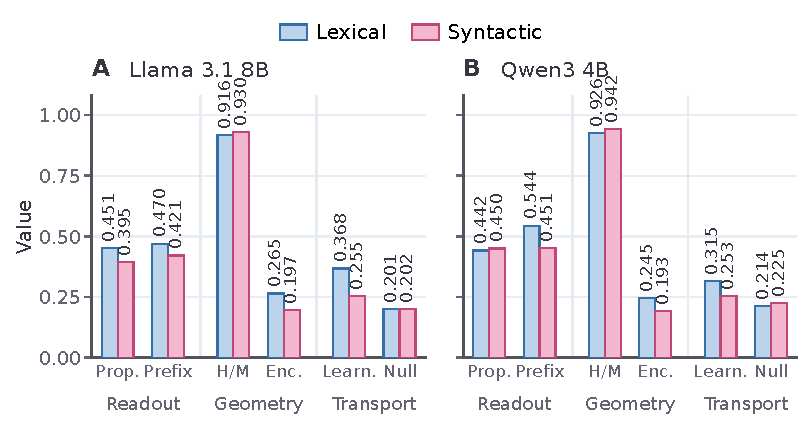
\includegraphics[width=\columnwidth]{figures/evidence_chain_summary.pdf}
    \caption{\textbf{Readout transfer and null-tested transport are distinct.} Llama (A) and Qwen (B) compare lexical and syntactic results across readout, direction alignment, and transport area.}
    % 中文图注：读出迁移与经过零假设检验的传输并不等同。Llama (A) 与 Qwen (B) 比较词汇和句法方向的读出、方向一致性与传输面积。
    \label{fig:evidence-chain}
\end{figure}

\paragraph{Lexical transport.} Llama lexical depth-normalized area is 0.368 against a null mean of 0.201; Qwen is 0.315 against 0.214. No complete null pipeline reaches either learned curve, yielding \(p=1/101=0.0099\) in both models. Learned-minus-null intervals are positive at every intermediate lexical checkpoint, and all 1,000 model--layer--sequence signed responses point machineward. This comparison preserves readout fitting, Jacobian translation, nuisance projection, and intervention trajectories; only the linguistic score-to-example correspondence is broken. The lexical effect therefore depends on that correspondence rather than on pipeline fitting alone.
% 中文：两个模型中的词汇传输都超过拟合流水线零假设。Llama 的词汇深度归一化面积为 0.368，零假设均值为 0.201；Qwen 分别为 0.315 和 0.214。没有任何完整零流水线达到两条学习曲线，因此两个模型均有 \(p=1/101=0.0099\)。每个中间词汇检查点上的学习方向减零假设区间都为正，全部 1,000 个模型—层—序列有符号响应也都指向机器方向。这一比较保留读出拟合、Jacobian 翻译、干扰投影和干预轨迹，只破坏语言得分与样本的对应关系。因此，词汇效应依赖于这一对应关系，而非仅由流水线拟合本身产生。

\paragraph{Transport contrast.} Syntactic signed response points machineward in 999 of 1,000 cases, and the source-side pullbacks agree strongly, but its depth-normalized areas of 0.255 in Llama and 0.253 in Qwen fall within the corresponding fitted-pipeline null distributions (\(p=0.1089\) and \(p=0.1980\)). The contrast identifies lexical realization as the component with correspondence-specific transport in both models. Construction alternatives, nuisance ranks, and fit counts appear in Figure~\ref{fig:app-hidden-robustness}.
% 中文：传输对比。1,000 个句法有符号响应中有 999 个指向机器方向，来源两侧的回拉也高度一致，但 Llama 与 Qwen 中 0.255 和 0.253 的深度归一化面积仍位于对应的拟合流水线零分布内（\(p=0.1089\) 与 \(p=0.1980\)）。这一对比把词汇语言实现识别为在两个模型中都具有对应关系特异性传输的成分。构造替代方向、干扰秩和拟合样本数分析见图~\ref{fig:app-hidden-robustness}。

Because lexical and syntactic axes pass the same surface and readout tests and enter the same intervention pipeline, their divergence isolates the role of the learned score-to-example correspondence. Every refitted null remains below the lexical curve, whereas 10 Llama and 19 Qwen null curves reach or exceed the syntactic statistic. The fitted null therefore selects a cross-model lexical trace rather than rewarding generic directional responsiveness.
% 中文：词汇与句法轴通过相同的表面与读出检验，并进入相同的干预流水线，因此二者的分化能够隔离学习到的得分—样本对应关系所起的作用。全部重拟合零假设都低于词汇曲线，而 Llama 的 10 条和 Qwen 的 19 条零曲线达到或超过句法统计量。因此，拟合零假设选择出跨模型的词汇轨迹，而不是奖励一般性的方向响应。

\paragraph{Construction robustness.} In all four model--axis cases, the canonical pullback has greater five-checkpoint capacity than upstream encoding, raw and nuisance-nullspace source contrasts, and the projected-random ensemble. Nuisance-rank and Jacobian-fit-count variants remain close to the frozen direction. These checks support a source-consistent pullback over simpler substitutes; the complete refitted null still determines the lexical headline result (Figure~\ref{fig:app-hidden-robustness}).
% 中文：在四个模型—轴组合中，规范回拉的五检查点容量都高于上游编码、原始来源对比、干扰零空间来源对比以及投影随机集合。干扰秩与 Jacobian 拟合样本数变体也保持接近冻结方向。这些检查支持采用来源一致回拉而不是更简单的替代方向；决定词汇主结果的仍然是完整重拟合零假设，详见图~\ref{fig:app-hidden-robustness}。

\begin{figure}[!t]
    \centering
    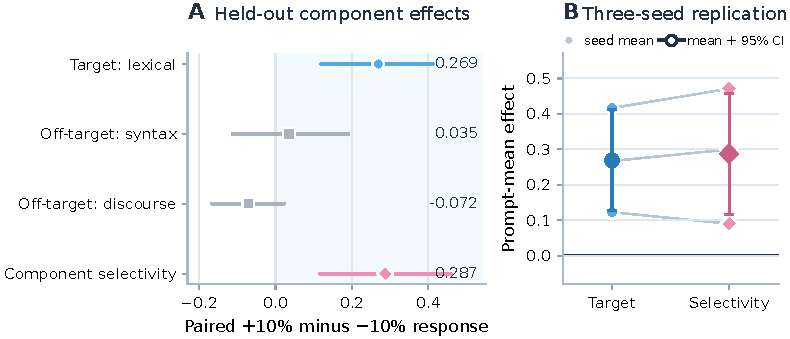
\includegraphics[width=\columnwidth]{figures/representation_realization_audit.pdf}
    \caption{\textbf{Held-out lexical control is target-aligned and selective.} (A) Target, off-target, and selectivity intervals. (B) Positive target and selectivity means in all three seeds.}
    % 中文图注：持出词汇控制与目标一致且具有选择性。(A) 目标、非目标与选择性区间；(B) 三个随机种子的目标与选择性均值均为正。
    \label{fig:audit}
\end{figure}

\begin{table}[tbp]
\centering
\maintablefont
\setlength{\tabcolsep}{2.5pt}
\renewcommand{\arraystretch}{1.08}
\begin{tabular*}{\columnwidth}{@{\extracolsep{\fill}}lrrr@{}}
\toprule
\textbf{Estimand} & \textbf{Mean [95\% CI]} & \(\boldsymbol{d}\) & \(\boldsymbol{p}\)\\
\midrule
Lexical target & 0.269 [0.127, 0.412] & 0.280 & 0.0006\\
Syntactic off-target & 0.035 [\textminus0.112, 0.191] & 0.035 & 0.6613\\
Discourse off-target & \textminus0.072 [\textminus0.167, 0.023] & \textminus0.114 & 0.1454\\
\graymidrule
Component selectivity & 0.287 [0.117, 0.459] & 0.255 & 0.0012\\
Target \textminus{} syntax & 0.234 [0.011, 0.457] & 0.162 & 0.0374\\
Target \textminus{} discourse & 0.340 [0.184, 0.496] & 0.325 & \(<0.0001\)\\
\bottomrule
\end{tabular*}
\caption{\textbf{Held-out Llama lexical intervention.} Three-seed prompt means over 166 test prompts; \(p\) is a paired sign-flip test.}
% 中文表注：Llama 词汇干预的持出结果。表中为 166 个测试提示上的三种子提示均值；\(p\) 为配对符号翻转检验。
\label{tab:generation-audit}
\end{table}

\paragraph{Selective generation.} The held-out Llama lexical test completes the chain (Figure~\ref{fig:audit} and Table~\ref{tab:generation-audit}). The target projection is \(0.269\,[0.127,0.412]\), with seed means 0.123, 0.267, and 0.416. Component selectivity is \(0.287\,[0.117,0.459]\), with seed means 0.090, 0.300, and 0.471. Syntactic \(0.035\,[{-}0.112,0.191]\) and discourse \(-0.072\,[{-}0.167,0.023]\) responses remain centered near zero. The target also exceeds syntax by \(0.234\,[0.011,0.457]\) and discourse by \(0.340\,[0.184,0.496]\). The prompt geometry and smoothed distributions appear in Figure~\ref{fig:app-generation-robustness}.
% 中文：选择性生成。Llama 词汇方向的持出检验完成了整条证据链（图~\ref{fig:audit} 与表~\ref{tab:generation-audit}）。目标投影为 \(0.269\,[0.127,0.412]\)，三个种子均值依次为 0.123、0.267 和 0.416。成分选择性为 \(0.287\,[0.117,0.459]\)，三个种子均值依次为 0.090、0.300 和 0.471。句法响应 \(0.035\,[{-}0.112,0.191]\) 与篇章响应 \(-0.072\,[{-}0.167,0.023]\) 仍以零附近为中心。目标还以 \(0.234\,[0.011,0.457]\) 超过句法，以 \(0.340\,[0.184,0.496]\) 超过篇章。提示级联合几何和平滑分布见图~\ref{fig:app-generation-robustness}。

\paragraph{Visible lexical change.} The aggregate projection corresponds to a concrete shift in one of the strongest source features. Relative to \(-2w\), \(+2w\) lowers function-word rate by \(0.0084\,[0.0038,0.0130]\) in magnitude, matching the machineward sign of the observational effect (\(d=-1.221\)). Pronoun rate and mean content-word frequency move in the same declared direction on average but have intervals crossing zero. The intervention therefore changes a distributed lexical score with one individually resolved realization, rather than depending on a single trigger word.
% 中文：可见的词汇变化。总体投影对应于最强来源特征之一的具体变化。与 \(-2w\) 相比，\(+2w\) 使功能词比例在幅度上降低 \(0.0084\,[0.0038,0.0130]\)，与观察效应的机器方向符号一致（\(d=-1.221\)）。代词比例与平均内容词频率在均值上也沿预先声明方向移动，但区间跨越零。因此，干预改变的是分布式词汇得分，并包含一个单独可确定的语言实现，而不是依赖某个触发词。

\section{Discussion}
% 中文：讨论

\paragraph{A controllable lexical coordinate.} The central result is an end-to-end correspondence: a distributed lexical pattern recurs under two elicitation interfaces, is continuously readable after generator holdout, transports beyond refitted nulls in two models, and selectively changes held-out Llama generations. The same frozen surface score defines every stage, so the final output effect is interpretable as movement of the original linguistic construct rather than an unrelated behavioral change. Development-set strength selection also shows why intervention scale belongs to the controller specification: the 10\% endpoint is fixed before the formal prompts and then replicated across three seeds.
% 中文：可控制的词汇坐标。核心结果是一条端到端对应关系：分布式词汇模式在两种诱导接口下复现，在生成器留出后仍可连续读取，在两个模型中都产生超过重拟合零假设的传输，并选择性地改变 Llama 的持出生成。每一阶段都由同一个冻结表面得分定义，因此最终输出效应可以解释为原始语言构念的移动，而不是无关行为变化。开发集强度选择还说明，干预尺度本身属于控制器规范：10\% 端点在正式提示之前冻结，并在三个种子上复现。

\paragraph{What the chain identifies.} The four stages progressively narrow the object of study. Surface recurrence identifies a corpus-level realization pattern; held-out readout locates an accessible coordinate that generalizes across generators; the fitted-pipeline null attributes transport to the learned linguistic correspondence; and paired generation establishes that the lexical response exceeds two measured off-target components. No stage is replaced by the next. Their conjunction is what permits a causal control interpretation while keeping the target anchored to observable language.
% 中文：证据链识别了什么。四个阶段逐步收窄研究对象。表面复现识别语料层面的语言实现模式；留出读出定位能够跨生成器泛化的可访问坐标；拟合流水线零假设把传输归因于学习到的语言对应关系；配对生成则证明词汇响应超过两个已测量的非目标成分。后一个阶段不会替代前一个阶段，只有它们的结合才能支持因果控制解释，并使目标始终锚定在可观察语言上。

\paragraph{Scope and implication.} Cross-model evidence is strongest through fixed-token transport; selective free-generation evidence is currently specific to the Llama lexical controller. Syntax remains readable but falls inside its fitted-null transport distribution, indicating that the method isolates component-dependent geometry rather than a generic source direction. This separation suggests a practical evaluation recipe for linguistic steering: define the surface construct first, verify held-out readout, test the complete learned pipeline against refitted nulls, choose intervention scale on disjoint development data, and reserve untouched prompts for target and off-target realization tests.
% 中文：范围与启示。跨模型证据在固定 token 传输阶段最强；选择性自由生成证据目前只针对 Llama 词汇控制器。句法方向仍可读取，但位于拟合零分布内，这表明该方法识别的是依赖语言成分的几何结构，而不是一般性的来源方向。这样的区分给出了语言引导的实用评估流程：先定义表面构念，再验证留出读出，随后用重拟合零假设检验完整学习流水线，在独立开发数据上选择干预尺度，并把未触碰的提示保留给目标与非目标实现检验。

\section{Conclusion}
% 中文：结论

We connect a corpus-conditioned lexical signature to selective generation. The direction recurs across generators and interfaces, remains readable after generator holdout, and transports beyond every refitted null in both Llama and Qwen. With strength selected on disjoint development prompts, the frozen Llama controller produces positive held-out target and component-selectivity intervals across three seeds.
% 中文：本文把依赖于语料的词汇特征连接到了选择性生成。该方向能够跨生成器和接口复现，在生成器留出后仍可读取，并且在 Llama 与 Qwen 中都产生超过全部重拟合零假设的传输。在独立开发提示上选择强度后，冻结的 Llama 控制器在三个种子上得到持出目标效应与成分选择性的正区间。
